\RequirePackage{fix-cm}
\documentclass[twocolumn]{svjour3}          % twocolumn
\journalname{Behavior Research Methods}


%\documentclass[jou,apacite]{apa6}
%\shorttitle{Online behavioral research with psiTurk}
%
%\twoauthors{Author One}{Author Two}
%\twoaffiliations{Institute of Psychology}{Freud's Institute}
%
%\abstract{psiTurk is really great and you should use it.}
%
%\rightheader{Online behavioral research with psiTurk}
%\leftheader{Online behavioral research with psiTurk}

\usepackage{listings}
\usepackage{color}
\usepackage{graphicx}
\usepackage{soul}
\usepackage{natbib}


\definecolor{dkgreen}{rgb}{0,0.6,0}
\definecolor{gray}{rgb}{0.5,0.5,0.5}
\definecolor{mauve}{rgb}{0.58,0,0.82}

\lstset{frame=tb,
  %language=Java,
  aboveskip=5mm,
  belowskip=5mm,
  showstringspaces=false,
  columns=flexible,
  basicstyle={\ttfamily},
  numbers=none,
  numberstyle=\tiny\color{gray},
  keywordstyle=\color{blue},
  commentstyle=\color{dkgreen},
  stringstyle=\color{mauve},
  frame=none,
  breaklines=true,
  breakatwhitespace=true
  tabsize=3
}

\begin{document}

\title{\textsf{psiTurk}: An open-source framework for conducting replicable behavioral experiments online}

% i set the authorship order based on github contributions
\author{Todd M. Gureckis$^1$ \and
	Jay Martin$^{1,2}$ \and
	John McDonnell$^3$ \and
	Alex Rich$^1$ \and
	Doug Markant$^4$  \and
	Anna Coenen$^1$ \and
	Jessica Hamrick$^5$ \and
	Patricia Chan$^1$
}


%\authorrunning{Short form of author list} % if too long for running head

\institute{
$^1$Department of Psychology, New York University\\
$^2$Stitch Fix, Inc.\\
$^3$Square, Inc.\\
$^4$Center for Adaptive Rationality, Max Planck Institute for Human
Development\\
$^5$Department of Psychology, University of California at Berkeley\\
\\
\textsf{psiTurk} was primarily written by the listed authors at the time the
first draft of this paper was constructed (version 2.0.0).  However, many people 
continually contribute to \textsf{psiTurk}'s evolving code base and
documentation via github.  
\\
\\
Please address correspondence concerning this paper to:\\
	Todd M. Gureckis \at
	New York University\\
	Department of Psychology \\
        \email{authors@psiturk.org}
}

\date{Received: date / Accepted: date}

\maketitle

\begin{abstract}
Insert your abstract here.
\keywords{Online experiments \and open science}
\end{abstract}

\tolerance=5000

\section{Introduction}


The ability to collect behavioral data from a large group of individuals
anonymously over the Internet has transformed the behavioral and social
sciences.  In addition to large scale experiments such as those
conducted by websites such as Facebook or 
Twitter~\citep[e.g.,][]{Chen:2013pb,Kramer:2014dq,Wu:2011sp}, many researchers
use online data collection to deploy ``traditional" experimental psychology
tasks.  The benefit of the online versions of traditional behavioral experiments include 
faster data collection and access to a potentially more diverse pool of participants. 
At the same time, conducting experiments online introduces a number of new 
technical and scientific challenges that must be addressed.

The project described in this paper, \textsf{psiTurk}, is an open-source framework of 
software and services that aims to address many of the technical challenges
involved in deploying experimental psychology experiments online.
It facilitates the creation, deployment, sharing, and replication of web-based experiments.
Study participants can be recruited via a number of methods including Amazon 
Mechanical Turk (AMT), which is currently the most popular platform for running 
paid human experiments online.

\begin{figure*}[tp]
\centering
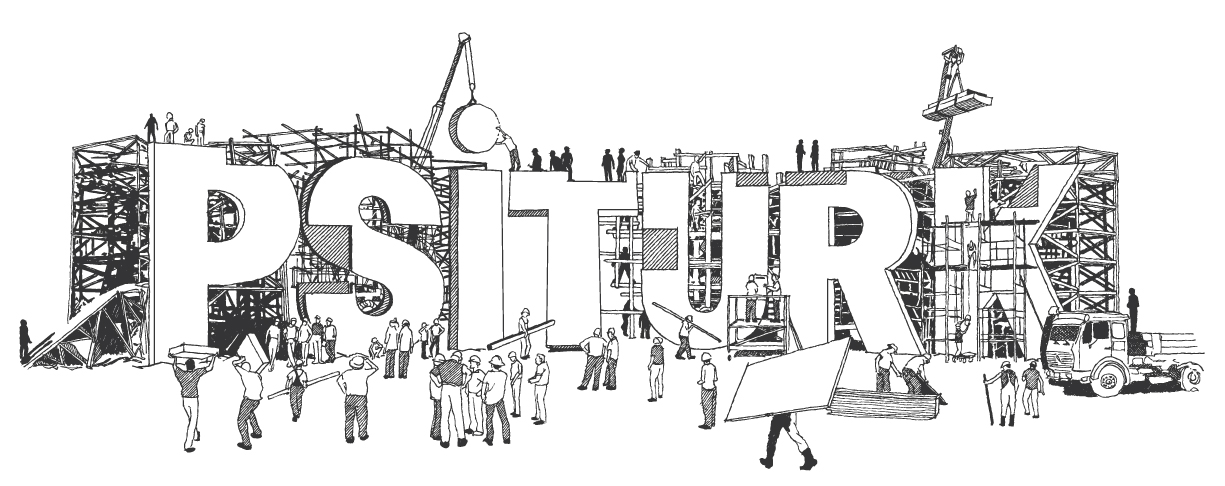
\includegraphics[scale=.30]{figures/psiturk_logo.jpg}
\caption{The \textsf{psiTurk} project is hosted on Github 
(http://github.com/NYUCCL/psiTurk) and at its main webpage (\textsf{http://psiturk.org}). 
The commissioned logo reflects the community-built orientation of the project.  A 
core philosophy is that better scientific software developed can be developed 
with more diverse input from many programmers~\citep{Raymond:1999zt}}.
\label{fig:logo}
\end{figure*}

To briefly summarize, \textsf{psiTurk} provides features for serving an 
experiment on the web, saving experimental data to a database, and restricting the 
participant pool according to the experimenter's needs (e.g., to prevent non-naive 
participants from contaminating a study). It also provides an interface with AMT to 
create and test new projects as well as to manage and pay participants. Finally, in 
the spirit of the recent ``open science" movement \citep{Collaboration:2012vf},
it provides  an open-source \emph{experiment exchange} for sharing experiments 
that can be easily replicated and extended by other researchers.  The code for 
\textsf{psiTurk} is open source, hosted publicly at
\textsf{http://github.com/NYUCCL/psiTurk} and interested researchers can easily 
contribute to improvements and bug fixes (see Figure~\ref{fig:logo}).

The principal goal of this framework is to handle common technical 
challenges so that researchers can focus on the development and replication
of online experiments.  In this paper we present a high-level overview of the 
\textsf{psiTurk} framework and its advantages for running web-based experiments.
In supplement to this overview, \textsf{psiTurk} provides a large and continually
evolving set of documentation hosted online (\textsf{https://psiturk.org/docs}).
We begin with an overview of the issues involved in online 
behavioral research,  the AMT platform, and the specific challenges that \textsf{psiTurk} is designed to 
address.  We then  step through the core functionality of \textsf{psiTurk} and 
describe its role in both an experimenter's and participant's workflow.  Finally, we
consider some future directions for \textsf{psiTurk} and online experimentation in 
general.



\section{The challenges of web-based experimental behavioral research}

\begin{figure*}[tp]
\centering
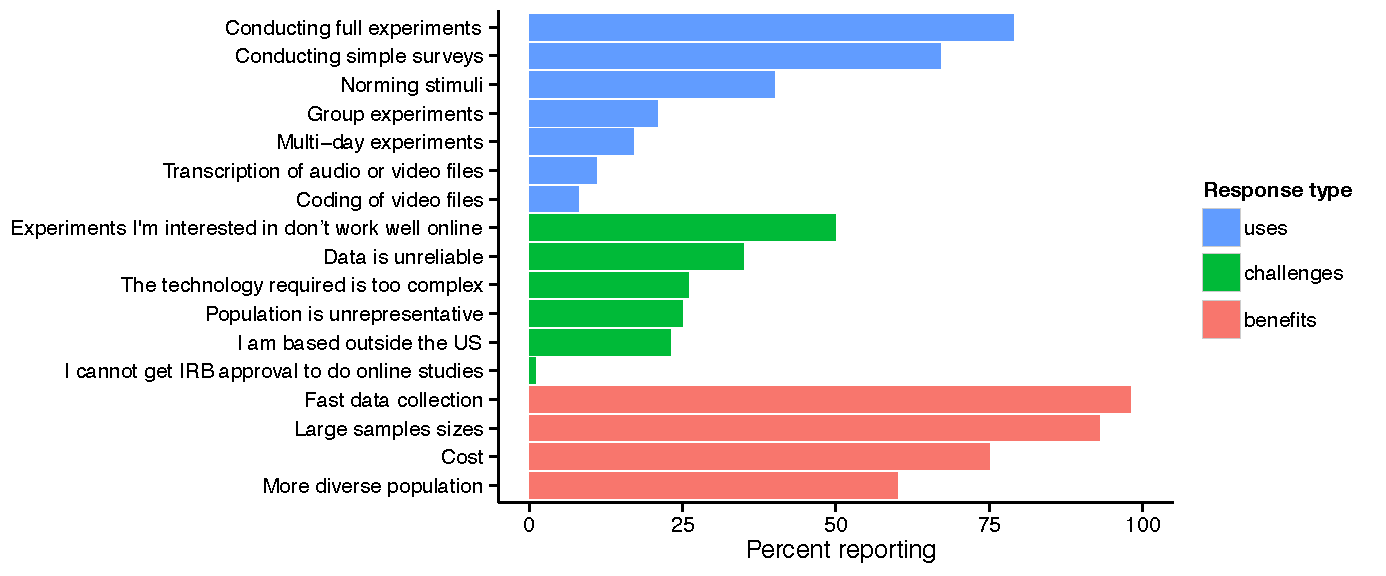
\includegraphics[width=\textwidth]{figures/combinedquestionsedited.pdf}
\caption{Reported uses, challenges, and benefits of online data collection as surveyed
by 201 behavioral researchers.}
\label{fig:survey}
\end{figure*}

It is easy to see why online experiments are an attractive option for behavioral 
scientists.  Compared to traditional methods of experimentation in the laboratory
they allow researchers to collect large data sets in a fraction of the time and at 
much lower cost (in terms of time, employment of research assistants, and typical 
compensation costs for participants).  Designing experiments for the web allows 
researchers to leverage the large set of software libraries developed to assist 
in the design of commercial web applications such as Node.js, JQuery, d3.js, 
and Boostrap.  Such libraries can be used to design the look and flow of an 
experiment in ways 
that far exceed the capabilities of traditional experiment running software developed 
in academia.  Such tools enable a wider range of experiments including more 
complicated interactive interfaces, or even multi-player games.

Still, there are a number of technical challenges to running experiments online.
For example, unlike in a laboratory setting, researchers have to 
deal with setting up a web server, recording data in a robust and secure way, 
and compensating participants over the Internet.  
Prior to the release of \textsf{psiTurk} version
2.0.0 (early 2014), we conducted an informal survey of behavioral researchers 
regarding their attitudes, concerns, and needs regarding online experimentation. 
To help introduce some of the core features and goals of \textsf{psiTurk} we 
quick summarize some of the findings from this survey



\subsection{Informal survey of the challenges researchers face conducting online experiments}
 We collected responses from 201 researchers in psychology (58\%),
linguistics (16\%), marketing (7\%), neuroscience (6\%), and economics (4\%), most of 
whom had some experience collecting behavioral data online in their labs (85\%).  
Respondents were recruited via mailing lists devoted to behavioral science and psychology 
as well as blogs and social media. 

The survey questions asked respondents about their attitudes and opinions towards
online data collection as well as the features they would look for in a software package
that helps with online data collection.  In the interest of brevity we highlight some of the
most important questions and answer.

Survey respondents showed a clear interest in online data collection. Nearly all listed fast data
collection and large sample sizes as benefits of online data collection, with most
interested in the potential for lower costs and a more diverse population as well 
(Figure~\ref{fig:survey}). Of researchers who had reviewed a paper which included data 
collected online, 59\% treated the data identically to data collected in the lab.


%\begin{figure*}[tp]
%\centering
%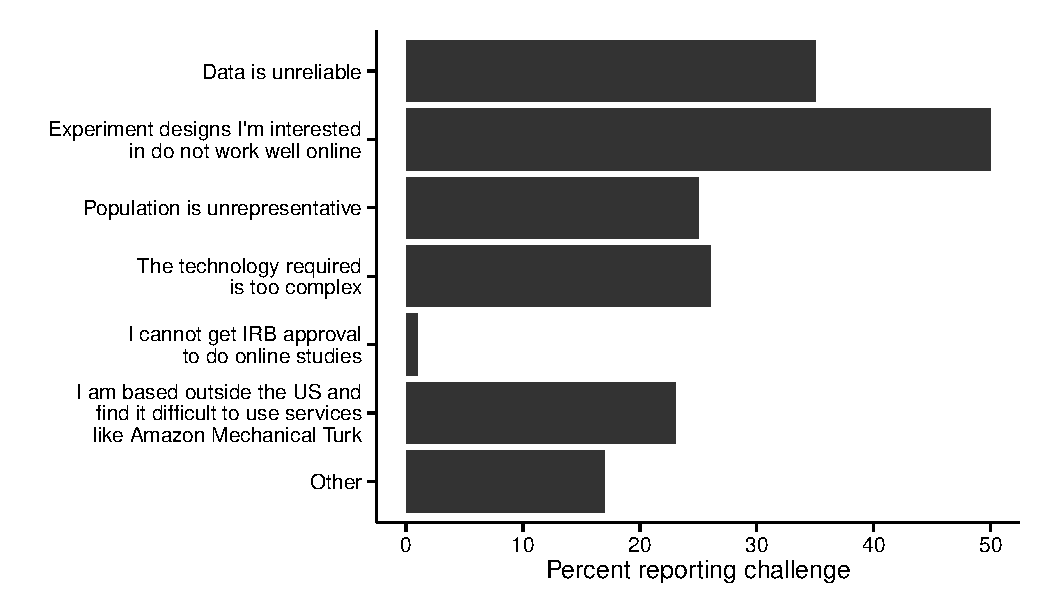
\includegraphics[scale=.75]{figures/challenges.pdf}
%\caption{Survey responses in answer to the question ``What are the major challenges 
% in using behavioral data collected online in research?" \hl{I suggest making this a full page 
% info graphic type thing that shows more of the interesting things in the survey that we 
% can use to open discussion of psiturk's features}}
%\label{fig:challenges}
%\end{figure*}

Respondents also felt that online data collected presented a set of unique challenges 
(Figure~\ref{fig:survey}).  Some felt that data collected online was unreliable or the
population unrepresentative. Many felt that experiment designs they were interested in did
not work well online, or that web technology is too complex, and researchers based
outside the US reported difficulty using services like Amazon Mechanical Turk.

\begin{table*}[tp]
\centering
\caption{Features the surveyed researchers desire in a software system for online data collection.}
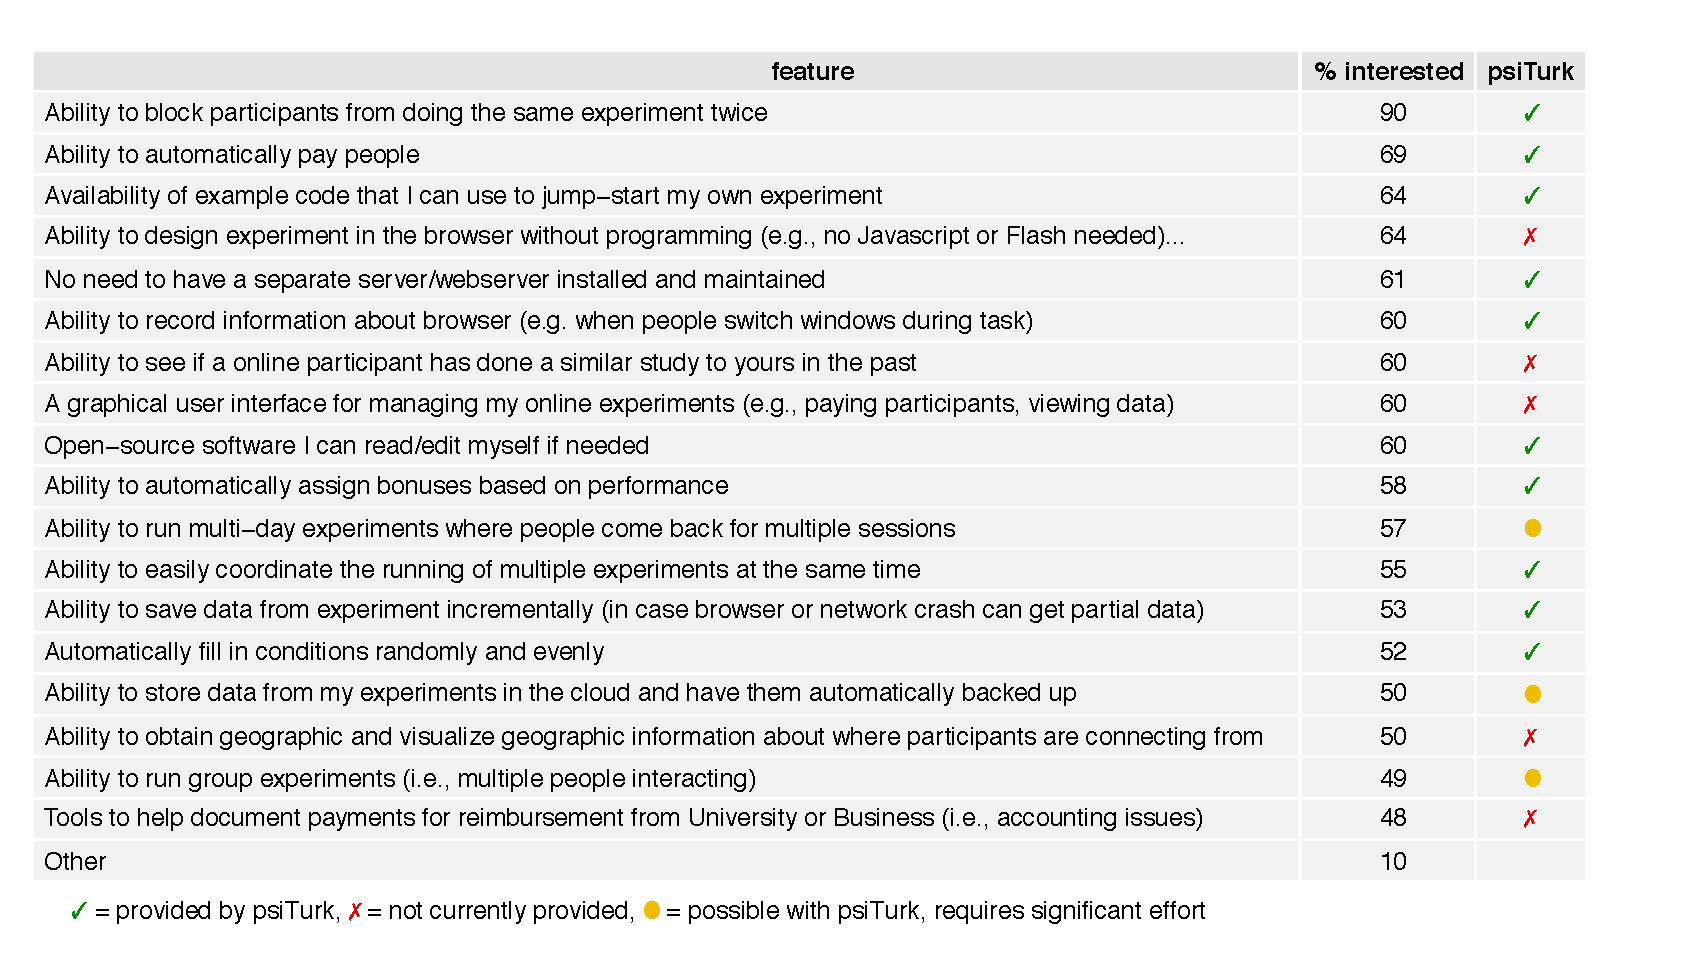
\includegraphics[width=\textwidth]{figures/featuresTable.pdf}
\label{tab:features}
\end{table*}


The majority of respondents (56\%) listed Qualtrics, a service for conducting online surveys, 
as the tool they were currently most likely to use, but most (79\%) expressed interest in 
being able to run full experiments including multiple, trials, fixation crosses, etc... 
(Figure~\ref{fig:survey}). The vast majority (94\%) reported interest in new tools that 
simplified online data collection. A full list of the features researchers are looking for in a 
online data-collection system are shown in Table~\ref{tab:features} (along with a checklist 
showing which are currently handled by \textsf{psiTurk}).  The important message is that
\textsf{psiTurk} successfully meets many of the major challenges the researchers identify.


\section{psiTurk and Amazon Mechanical Turk} 

Although allowing recruitment through a variety of methods (e.g., it can be
used to run experiments in a traditional lab setting),
\textsf{psiTurk} was primarily designed to facilitate online data collection using
the Amazon Mechanical Turk (AMT) crowdsourcing platform.
\cite{Mason:2012xy} provide a general overview of AMT features of
interest to academic researchers.  A key feature of AMT is that it provides a way for researchers
to easily recruit and compensate individuals for online experiments.  
People who complete tasks (called Human Intelligence Tasks or \emph{HITs}), are 
called \emph{workers}, and people who post tasks are called \emph{requesters}.
Beyond providing a platform to connect requesters and workers, AMT places few restrictions 
on the type of work that can be requested and the amount paid per HIT.  Workers are 
paid a fixed amount for each HIT they complete which is determined by the requester and
can be offered bonus payments for good performance.

From a worker's perspective, the AMT website provides an up-to-date listing of HITs that 
are available, with a title, brief description, and payment amount.  A worker can click on a HIT to 
see its full \emph{advertisement} (an embedded webpage that is either hosted by
Amazon or the requester) and decide to accept the HIT. 
Accepting a HIT reserves the ability to complete it within a timeframe specified by the requester.
The HIT is then be completed either on a requester's own hosted service (i.e., a webpage 
external to the AMT site), or on the AMT website itself through the use of customized templates.
Upon completion, the worker ``submits" the HIT, after which point the completed work must 
be approved by the requester before they are compensated.
In addition, some HITs offer bonus payments that are determined by the requester based 
on a worker's performance.

From a requester's perspective, AMT provides a web-based interface for creating/managing 
HITs and approving work that has been submitted.  In addition, they offer a ``sandbox" version 
of the platform in which HITs can be tested without paying live participants.
For basic tasks like surveys and open text fields, AMT offers a range of built-in templates that 
can be used to create experiments within the AMT website.  However, the degree of customization 
is limited for these templates. In particular, they do not support advanced experimental logic that is 
common to many psychology experiments (e.g., adapting the presentation of stimuli based on 
performance, or counterbalancing across a number of experimental variables).
In addition, they are limited to relatively simple forms of interaction and stimulus presentation.

For more complex tasks, a requester can provide a link to their own hosted web page or
web application which runs the 
experiment, saves the data, and only interfaces with AMT at the beginning of the task (receiving 
basic information about the worker) and at the end of the task (sending confirmation that the task 
has been completed).  Thus, these ``external HITs" enable a much wider range of experiments at 
the cost of additional technical requirements.  \textsf{psiTurk} is designed to handle many of the 
complex requirements associated with ``external HITs" so that researchers can more efficiently run 
these types of tasks.
% Specifically, it allows you to:
% 1. Run a web server for your experiment
% 2. Test your experiment
% 3. Interact with AMT to recruit, post HITs, filter, and pay participants (AMT workers)
% 4. Manage databases and export data



\section{What technical challenges is \textsf{psiTurk} designed to solve?}

The \textsf{psiTurk} platform is design to mitigate several of the technical complexities
involved in online experimentation, particularly using AMT.

\subsubsection{Web server and database management} 
To collect experimental data on the web, or specifically to run an external HIT on AMT, 
researchers minimally need a web server and database.  
The role of a web server is to respond to requests from participant's Internet browser 
for the experiment content.  The role of the database is to save the data provided by 
the participant.  Although less common in laboratory experiments, databases are 
necessary for online studies because it is impossible to save data to a participant's 
computer using a web page or web application (data must be stored on the server
rather than the client).  In addition, multiple participants often complete an 
experiment concurrently which can cause file corruption on certain system.  
Databases are specifically designed to manage concurrent reading and writing.
 
Setting up a webserver and database can be complex.  Some university Information
Technology departments
provide these types of services while the technical infrastructure at other 
institutions is lacking.  \textsf{psiTurk} includes a custom webserver and database
as a basic feature of the software tool which can be run from any computer
including a standard office computer or laptop.  This allows data collection from
anywhere without the need for a dedicated server computer.  In addition, \textsf{psiTurk}
can be easily installed on free hosting services such as Amazon Web Services
or RedHat's OpenShift.  Data collected with \textsf{psiTurk} is stored at a location
chosen by the experimenter and never visible to the \textsf{psiturk.org} cloud
services or Amazon, protecting the privacy of participants and helping with IRB compliance.

An additional complication is that contemporary web browsers are increasingly security
focused.  In particular, certain browsers will not load content that is not properly 
signed with a SSL certificate and accessed with a \textsf{https://} request.  This
is often difficult to obtain from universities and can be costly from online
hosting companies.  

\textsf{psiTurk} solves this later problem on behalf of researchers
using a cloud-based ``ad server" which will present securely signed
content for users.  One way to think of the ad server is as a digital
version of a ``bulletin board" which might be used to hang fliers
advertising particular studies within a university.  \textsf{psiTurk}
posts hosts the text of an ad using a unique URL.  Requests to access
this URL (usually from within the AMT system) are securely sent
the worker's browser.  If the worker decides to accept the HIT and
perform the experiment after seeing the ad they are forwarded to
the researcher's local computer to complete the task (it is up to the
experimenter if this later content is encrypted or not). Thus, 
the \textsf{psiTurk} ad server acts as a bridge between AMT and 
a researcher's local computer (see Section X for further information 
about the ad server). 


\subsubsection{Communicating with AMT}

When using AMT to recruit and compensate participants,
experimenters typically use the AMT website.  This often
involves a lot of manual, error-prone clicking.   \textsf{psiTurk}
essentially has automatically scripted many of the common
tasks that researchers have to do on AMT's website such
as pay all participants, assign bonus, check the current
account balance, and monitor the progress of an experiment.
This is accomplished via an interactive UNIX-based command
line tool (see below).
The goal of this tool is to help prevent errors in payments and
to save researchers considerable time.

\subsubsection{Programming an experiment}
\textsf{psiTurk} provides a number of features which help researchers implement 
experiments.  These include a Javascript library (psiturk.js), basic HTML templates 
for commonly used components such as consent forms and instruction screens, 
and an user-contributed ``experiment exchange" where researchers can share the code for their \textsf{psiTurk}-compatible
projects (\textsf{http://psiturk.org/ee}). 

The psiturk.js javascript library provides basic functions of recording data and sending it back to the psiturk server,
preloading pages and images, as well as some basic functions for looping through instructions
screens and providing (and recording) informed consent.
However, the \textsf{psiTurk} framework is \emph{not} designed as a generic
programming interface for building 
experiments (e.g., it does not provide code for widgets such as sliders or buttons) and assume
researchers will use some basic Javascript, HTML, and CSS to design their experiment.  Instead, \textsf{psiTurk}'s
philosophy is that general purpose javascript libraries available online for creating dynamic content (e.g., jquery or
Twitter's Bootstrap library) provide the most powerful and well-documented set of features.  Instead, \textsf{psiTurk}
aims to help share code and propagate ``best practices" among the research community.
This later goal is supported by the online ``experiment exchange.'
The source code for projects in the exchange can be downloaded and modified for a new use,
replicated directly, or can simply provide example of code implementing a particular 
feature.  In addition to the exchange, \textsf{psiTurk} also includes with a complete working example 
experiment that can be used as a template for new projects.

%That is, it requires that the experimenter knows some basic JavasScipt, HTML, and CSS to code the logic and looks of a new study.


\subsubsection{Recruiting, filtering, and instructing participants}
Finally, \textsf{psiTurk} has a number of features for controlling the recruitment
of participants which can contribute to higher quality control.
For example, \textsf{psiTurk} offers basic capabilities for assigning workers to different experimental conditions 
and counterbalancing different aspects of the experiment.
In addition, it allows experimenters to filter workers in particular ways.  For example, using \textsf{psiTurk}
is it possible to exclude participation by workers user certain devices (such as phones or tables) or browsers
which are known to have compatibility issues with the experimenter's design (for example restricted
users of Firefox or Internet Explorer).  \textsf{psiTurk} also allows researchers to prevent a AMT worker from 
participating in the same experiment more than once (which might otherwise be tempting when
large financial rewards are offered).  Future version of \textsf{psiTurk} may also allow researchers to 
block AMT workers who have completed certain \textsf{psiTurk} experiments in the past such as
preventing anyone who has already completed a similar experiment~\citep[see][for a discussion about non-naivety amongst AMT workers]{chandler2014nonnaivete}.


With these general features in mind, we now turn to a more detailed overview of the 
\textsf{psiTurk} platform.

\begin{figure*}[tp]
\centering
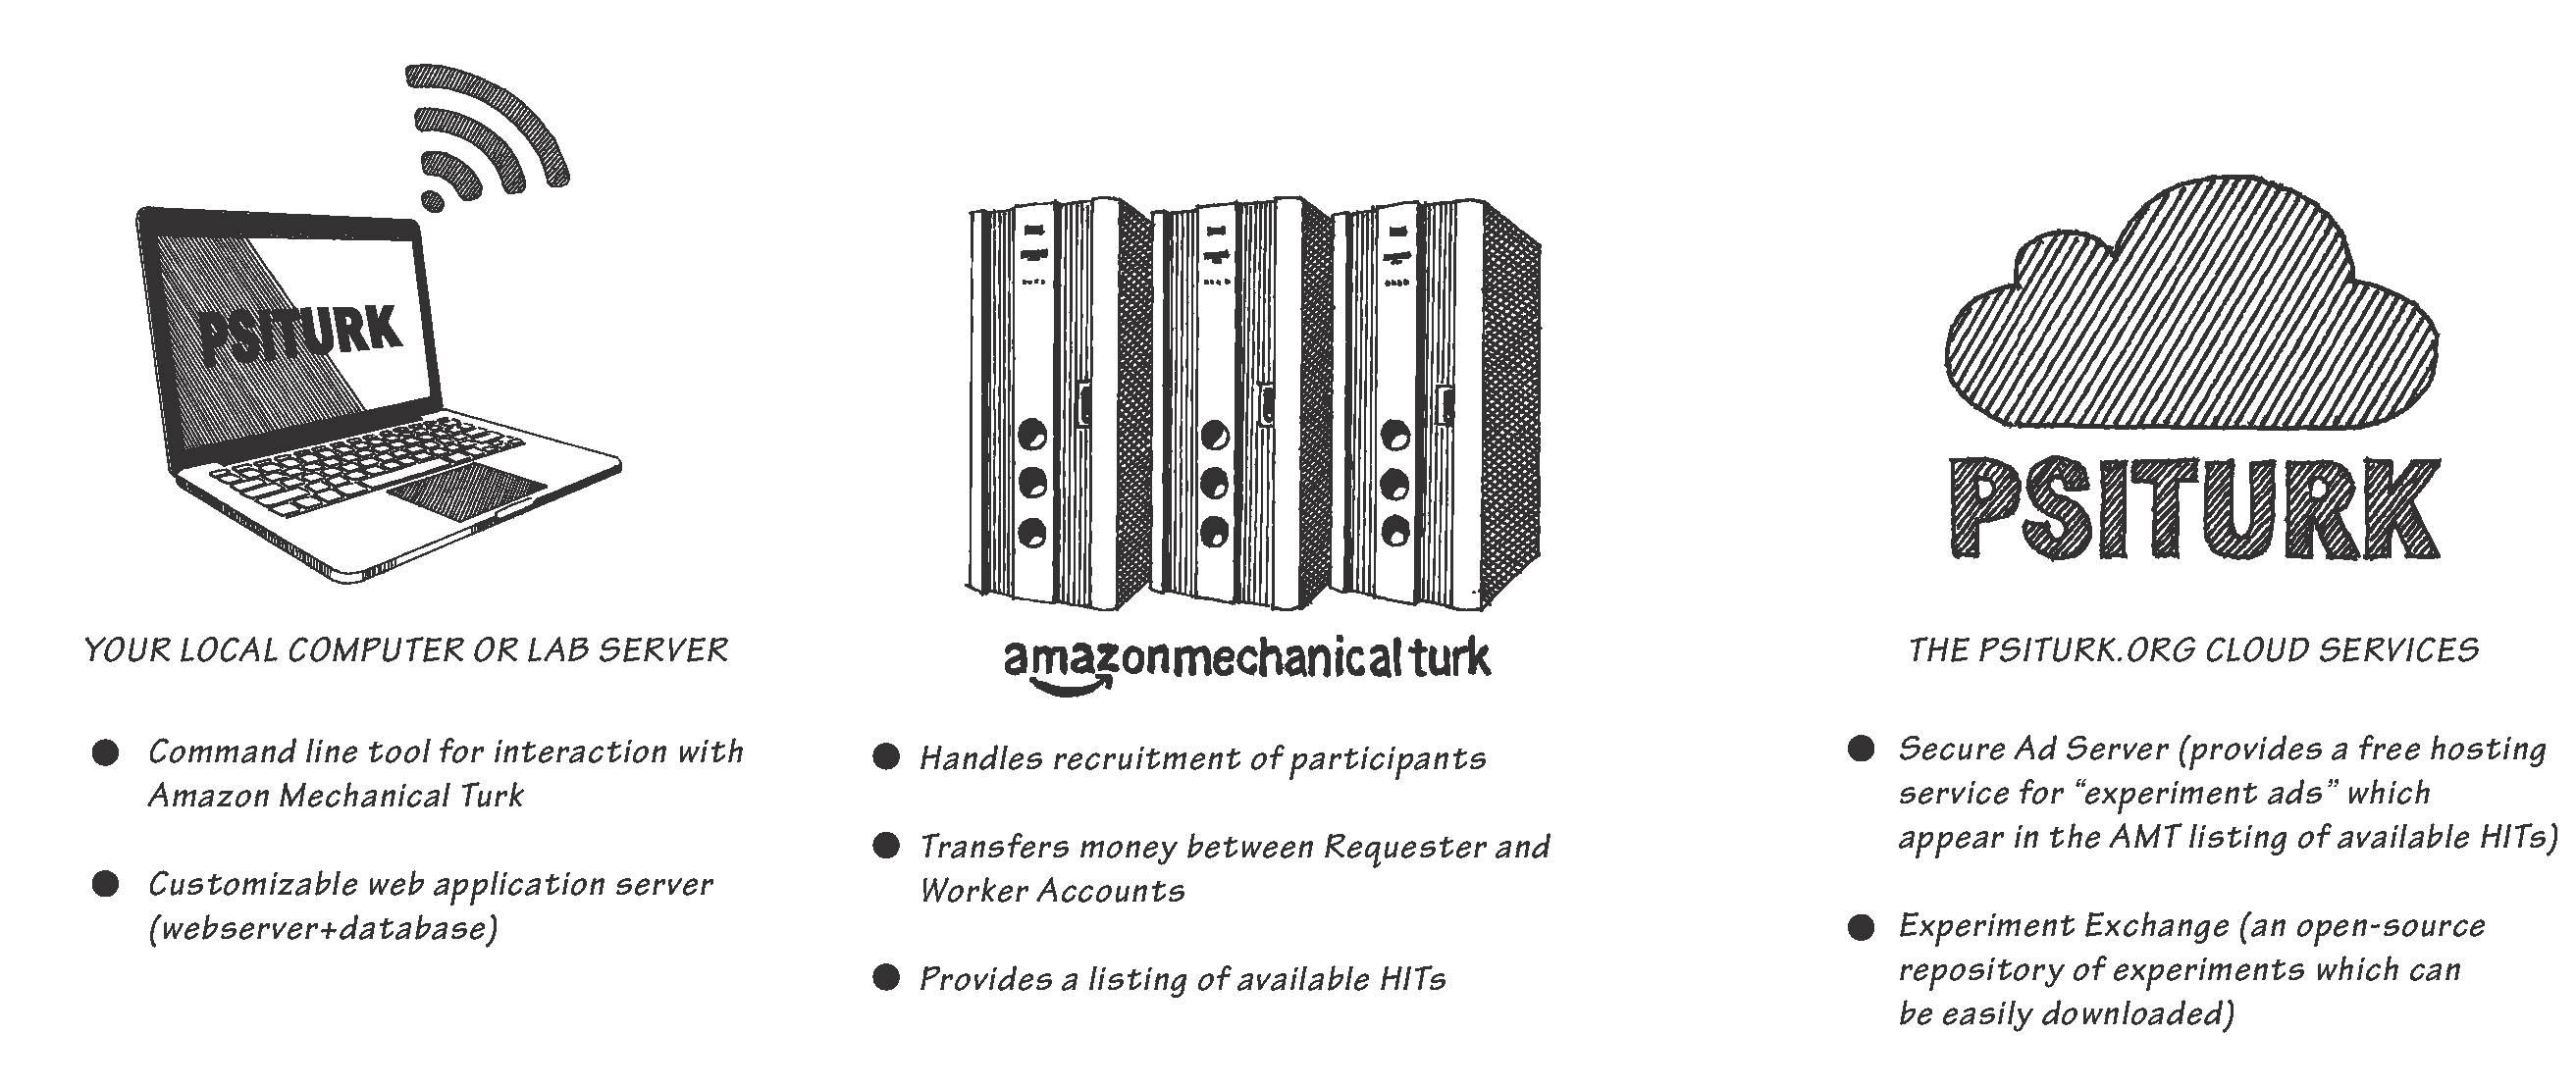
\includegraphics[scale=.40]{figures/psiturk-components.pdf}
\caption{Three key components of the \textsf{psiTurk} system.  }
\label{fig:components}
\end{figure*}


\section{Key components of the \textsf{psiTurk} platform}

The overall structure of the \textsf{psiTurk} platform is shown in Figure~\ref{fig:components}
and can be conceptualized as involving three components.
First, there are a collection of software tools which run locally on a user's
local computer or server.  These local components include a command line tool and 
a web application server (which provides both a customizable webserver and 
database solution).  Next, \textsf{psiTurk} relies currently on Amazon
Mechanical Turk to handle the recruitment and compensation of participants.
Finally, the \textsf{psiturk.org} cloud based component includes a hosted ``ad server" 
and the experiment exchange.  In the following sections we highlight the important 
functions of each component.

\subsection{Local computer or server}

\subsubsection{Command line tool}

When using \textsf{psiTurk}, the researchers 
local computer (laptop, lab server) runs the \textsf{psiturk} 
interactive UNIX-based command line tool.  
This tool is used to issue commands and interact
with the Amazon Mechanical Turk system and with the \textsf{psiTurk} cloud.  
The design choice of a command line interface was 
selected to make it easier to add new functionality to the system quickly (without 
needing to design time consuming GUI elements), thus the set of
available commands continues to grow.
Example uses of the command line tool include checking the user's Amazon
Mechanical Turk account balance, paying participants, and creating new HITs.
The command line has the capability to give automated bonus payments to 
participants based on a function designed by the experimenter. This feature is 
particularly helpful since the AMT website requires bonuses to be entered by hand 
for each participant individually.


\subsubsection{Web application server (webserver + database)}

The command line tool is also used to interact with the web application server.
The web application server handles the logic determining which pages to show
to a participant at different stages of the experiment.  \textsf{psiTurk} comes with
a default web application which implements many important features commonly
needed by experiments (e.g., checking that a user hasn't already done the experiment,
recording and saving data to a centralized database).  In addition the web application
server can be heavily customized to include more complex types of experiments.
For example, in one instance we made an experiment where a cognitive model
is fit to participants data in real time and used to determine the sequence of future
trials in the experiment.  The logic for the model fitting was done within the 
web application system itself rather than coding all of this mathematics in
Javascript.

\subsection{Amazon Mechanical Turk and Amazon Web Services}

 Amazon Mechanical Turk's servers handle the recruitment of participants via
its crowdsourced labor force.  It also handles the transfers of money between Requesters and
Workers.  Finally, it provides a listing of available HITs which workers can browse through looking
for interesting work.  Amazon Mechanical Turk is one part of a larger collection
of cloud-based services provided by Amazon via the Amazon Web Services.
For example, using the \textsf{psiTurk} command line tool users can create a
database server running on Amazon's cloud with a few short commands.  This database
can then be used instead of a local database solution.

\subsection{\textsf{psiturk.org} cloud services}
In addition the command-line tool and the web application server, \textsf{psiTurk}
provides a few services that run on a constantly available web server.
Most important of these is that psiTurk "Secure Ad Server."  When a user
creates a new HIT and wishes to post it to AMT, typically one advertises the
study to potential participants (explaining how long the task will take and how
much it will pay).  As mentioned earlier, these "ads" will not correctly display
in worker's browsers unless they are encrypted using SSL.  The \textsf{psiturk.org}
ad server allows users of the psiturk system to host ads on the \textsf{https://psiturk.org}
website which are encrypted.  These ads are what appear in the browsable listing
on the Amazon Mechanical Turk website.
As mentioned earlier, the psiturk Experiment Exchange provides
a open-source repository of \textsf{psiTurk}-compatible experiments which can be 
easily downloaded.  The coordination of these downloads is handled by the \textsf{psiturk.org} cloud.

%Complete documentation and tutorials are available at http://psiturk.org/docs, including instructions for installing the software.

\section{Requirements and initial setup - (AC)}

\hl{can someone work on requirements?}
% this needs to cover
% 1. creating AMT account (maybe just mention necessary and provide link to instructions
% online someplace because will be outdated by time anyone reads this
% 2. create psiturk.org account

After creating an Amazon Web Services account, a researcher must obtain credentials (a \emph{key ID} and a \emph{secret key}) that are then added to a global configuration file \texttt{.psiturkconfig}.
When psiTurk runs for the first time this file is automatically created in the user's home directory, but the user's AWS credentials must be added in order for psiTurk to interact with AWS.
Additionally, an account (and associated pair of keys) on the psiTurk.org website is required to allow posting of ads on the Ad server.
These credentials (obtained from a user's psiTurk profile page) are also placed in \texttt{.psiturkconfig}.

This global configuration is used whenever psiTurk is run, allowing multiple experiments (each residing in its own directory somewhere on the user's system) to rely on the same AWS and psiTurk accounts, or to share other common configuration options as desired.


% 3. install psiturk via pip (maybe describe system requirements, minimum python version)
% 4. discussion optional database option

\section{Getting started with \textsf{psiTurk}}

The following section provides a basic overview of how to use psiTurk,
explaining the various steps required of new users of the system along with
some details about how the various components described above interact.

\subsection{Configuration and project structure - (AR)}

A new \textsf{psiTurk} project can be initialized in the current directory using:

\begin{lstlisting}
$ psiturk-setup-example
\end{lstlisting}

\noindent which creates a new directory containing an example experiment.
This example can be a template for building more custom designs.
The project directory typically includes the following files: \\


\noindent \texttt{config.txt}: This file contains settings for the current experiment, including:

\begin{itemize}
\item Metadata about the experiment that is displayed to workers on the AMT website (title, description)
\item Restrictions on which workers can accept the HIT, including geographic location (e.g., limiting to US workers only), AMT-specific qualifications (e.g., a worker's proportion of past work that has been approved), and web browsers that are permitted.
\item Database setup (Sqlite by default)
\item Server parameters (URL, port number)
\item Task parameters (e.g., number of conditions)
\end{itemize}


\noindent \texttt{custom.py}: Within Flask web framework, possible to add custom routes so that server-side functionality can be added to the psiTurk web server. \\ 

\noindent \texttt{participants.db}: If Sqlite is used (on by default), this file will be the database. \\

\noindent \texttt{server.log}: A log file containing any messages from the experiment server (not from the actual experiment code!) \\ 

\noindent \texttt{static/} directory: Experiment files, including Javascript, CSS, and images. \\

\noindent \texttt{templates/} directory: HTML files associated with experiment \\


Setting up a new experiment thus entails 1) editing the settings in \texttt{config.txt}, and 2) modifying the contents of the \texttt{static} and \texttt{templates} directories to program the experiment.
The remaining files are only necessary in order to debug server errors (\texttt{server.log}), add new server-side functionality (\texttt{custom.py}), or to access saved data (\texttt{participants.db}).

Creating the experiment requires at least some basic web programming skills (especially using HTML, CSS, and JavaScript).
Once you mastered the basics, you can take advantage of the vast number of libraries and tools that can help you to build sharp and sophisticated experiments with the support of a large community of users.


\subsection{Command line interface: Managing HITs and serving the experiment - (AR)}

PsiTurk runs as a command line interface (CLI) within a standard terminal window.
There are several advantages to designing psiTurk as a simple CLI beyond its efficiency of use. This
design makes the user-interface code clear and easy to read and write, allowing newcomers to quickly
understand and contribute to the open-source project. Integrating a new feature into the interface
is as simple as describing the syntax and functioning of a new command. The CLI also ensures that
psiTurk is easy to interact with not just on a laptop or desktop but also on a remote server or in
the cloud, where users may have terminal-only access.
 
Tab completion makes it quick to type commands, and the \texttt{help} command can be used to show
details on the usage of any command. 
The straightforward and consistent syntax of the CLI allows
users to perform a wide variety of tasks--from creating HITs and paying workers, to launching Amazon
Web Services database instances, to opening an experiment in a browser for debugging--that
would otherwise be spread across a number of websites and programs. 

Entering
\texttt{psiturk} at the command line in any directory containing a psiTurk project launches the
psiTurk CLI.
The psiTurk CLI features a colorized prompt that provides important information at a glance, including
whether the server is running, the current mode (``live" or ``sandbox", and the number of HITs currently running on AMT:

\begin{lstlisting}
[psiTurk server:off mode:sdbx #HITs:0]$
\end{lstlisting}

\noindent In some examples below, this prompt is truncated as \texttt{[psiTurk]\$} to indicate commands that occur within the psiTurk CLI, while commands that are entered on the command line are preceded simply by \texttt{\$}.


\subsubsection{Managing HITs}
Commands are organized into groups based on their function, following a general ``\texttt{command subcommand
arguments}'' format. For example, one can create a HIT by typing 

\begin{lstlisting}
[psiTurk]$ hit create <# assignments> <$ amount> <duration>
\end{lstlisting}

What happens after you create a HIT?

List any existing HITs with:

\begin{lstlisting}
[psiTurk]$ hit list --active
\end{lstlisting}


\subsubsection{Serving an experiment}

The experiment server is started using

\begin{lstlisting}
[psiTurk]$ server on
\end{lstlisting}

\noindent This opens the port specified in the project configuration file.
The experiment server will then respond to incoming requests, assuming that the port is publicly accessible.
This requires a static IP to prevent the experiment's URL from changing.
Users without a static IP address can use a dynamic DNS service to forward requests to their dynamic IP.
If the system running psiTurk is behind a router, the router must be configured to forward requests on the same port.

During the development of an experiment, the current code can be tested using:

\begin{lstlisting}
[psiTurk]$ debug
\end{lstlisting}

\noindent which will open a new browser window in which the current experiment can be tested.

Can restart the server with \texttt{server restart} or open the server log with \texttt{server log}. 

The sandbox mode is active by default, which means that calling \texttt{hit create} will submit a HIT to the AMT sandbox website.
The experimenter can then test the experiment from the perspective of a worker before making it publicly available.
Once the experiment is ready for real workers, the \texttt{mode} command can be used to switch to ``live" mode, after which newly created HITs will be submitted to the main AMT site.

In most cases, a user of the
psiTurk CLI will never have to log into the MTurk website except to add money to their MTurk
requester account.


\begin{figure*}[tp]
\centering
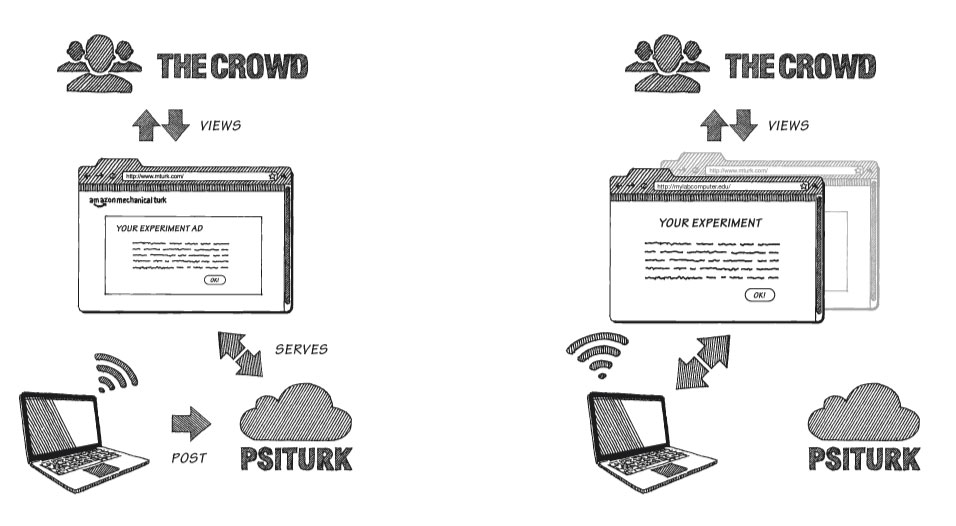
\includegraphics[scale=.40]{figures/psiturk_cloud_sequence.jpg}
\caption{How the ad server works.}
\label{fig:adserver}
\end{figure*}


\subsection{The secure ad server - (TG)}

\textsf{psiTurk} provides a cloud service at \texttt{psiturk.org} for serving ads to workers.
This service serves the ads with appropriate SSL certificates, something which can be difficult on many server configurations.\footnote{SSL certification has recently become a requirement for hosting content within an \texttt{iframe} on \texttt{mturk.com}.}
The Ad Server removes need to deal with complex web security issues (https, data mining on workers) 
Participants recruited via Mechanical Turk first interact with your task via ads. Ads are simply the digital version of hanging a poster or flyer around your university building in order to recruit participants. Technically, ads are snippets of HTML code that describe what your task is about and what you're offering for compensation. As a result, they are the front line for any subject recruitment online. It's easy to overlook the importance of a good ad, and making that ad visible to as many participants as possible.


%Second, the PsiTurk web framework allows you to easily build and host your own experiment, running on your server or laptop and saving workers' data either to your own database  or to \texttt{psiturk.org}.
%This gives experimenters complete flexbility in terms of content while also offering a suite of tools to make experiment development easy.



%Extendable Python based API: easily add new functionality
%
%Library of experiments you can adapt or replicate
%
%Fully open-source development helps catch bugs
%
%Since everything runs locally easy to debug/test (even w/o Internet!)
%
%Run experiments on local computer (via tunnel) (can run offline and online)
%
%Perfect for laboratory-based courses with undergrads (replicating studies)



\subsection{Javascript library \emph{psiTurk.js}}

The javascript library \emph{psiTurk.js} enables interaction with the server from the client-side (javascript) experiment code.
The goal of the library is to handle the most common functionality of psiTurk-based web experiments, without imposing any additional requirements on the structure or design of the experiments themselves.
Researchers can draw on a vast array of javascript libraries to design their experiment, while using psiTurk.js to save data and notify the server of changes in a participant's status.

\subsubsection{Initialization}

Figure X shows javascript code from an experiment script (\texttt{static/js/task.js}). 
Initialization. 
Preloading of HTML and images.
Basic structure for presenting instructional pages.

\subsubsection{Tracking a participant's progress in an experiment} 

psiTurk records changes in a participant's status as they move through an experiment. 
Some of these status changes are automatic, e.g., when a participant is assigned to a condition or if they quit an experiment early. 
Two additional status changes are initiated by the client-side experiment code using psiTurk.js functions.
First, since experiments typically begin with an instructional phase, calling the function \texttt{psiturk.finishInstructions()} upon completion of this phase will save the participant's status as having begun the main experiment.
If the participant attempts to quit the experiment after that point, they will receive a warning that they will not be able to restart the experiment and may forgo payment.
Second, successful completion of the experiment is signaled by calling \texttt{psiturk.completeHIT()}, which closes the experiment and redirects the participant to the AMT page to submit their HIT.

\subsubsection{Saving experimental data} 

Experiment code can save data in two formats.
\texttt{psiturk.recordTrialData} takes any list of values as input and appends it to a list of ``trial" data.
This data structure is meant for sequential data that may be collected over the course of multiple trials or blocks, where each line corresponds to a new measurement.
However, the format of this data is defined by the experimenter and is saved in the database as a single JSON object.

In contrast, \texttt{psiturk.recordUnstructuredData} is used to record (key, value) pairs, where the key is uniquely defined within the experiment.
This format is useful for survey questions or other one-time measurements, e.g., (\emph{Age}: 24).

Importantly, both functions above simply record the data in the appropriate format on the client-side.
When the experimenter wishes to save the data to the server they call \texttt{psiturk.saveData()}, at which point both sets of data are sent to the server to be recorded in the database.

\subsubsection{Automatic recording of browser interaction}
 
One general shortcoming of web experiments is greater uncertainty about a participant's testing environment and engagement with the experiment.
Unlike lab computers where most undesired behaviors can be prevented, a web participant is always able to close a web browser, switch to different applications, or change other aspects of their experience.
However, standard methods exist for recording many aspects of a user's interaction with a web browser, and this data can be useful for 1) tracking how an experiment was actually displayed, and 2) the level of a participant's engagement.

For example, although it is possible to set the initial size of a browser window, a web participant can change the dimensions of the window, potentially obscuring or altering how the experiment is displayed.
\emph{psiTurk.js} automatically records these changes in the size of the window.
Similarly, the experiment can choose to switch focus away from the experiment window (e.g., to another browser window or a different application).
\emph{psiTurk.js} automatically records every time that the experiment window loses and gains the participant's focus.
This ``event data" is automatically recorded and saved to the database whenever \texttt{psiturk.saveData} is invoked. \\





\begin{lstlisting}[float=*,numbers=left,numberstyle=\small\color{gray},caption=Example experiment code (javascript)]
// Initalize psiturk object with parameters passed from server (see templates/exp.html)
var psiTurk = new PsiTurk(uniqueId, adServerLoc, mode);

var mycondition = condition;  // these two variables are passed by the psiturk server process
var mycounterbalance = counterbalance;  // they tell you which condition you have been assigned to

// All HTML snippets to be loaded from templates directory
var pages = ["instructions/instruct-1.html", ...];
psiTurk.preloadPages(pages);

var StroopExperiment = function() {
	...	
	var response_handler = function(e) {
		...
		if (response.length>0) {
			listening = false;
			var hit = response == stim[1];
			var rt = new Date().getTime() - wordon;

			psiTurk.recordTrialData({'phase':"TEST",
                                     'word':stim[0],
                                     'color':stim[1],
                                     'relation':stim[2],
                                     'response':response,
                                     'hit':hit,
                                     'rt':rt}
                                   );
			remove_word();
			next();
		}
	};
	...	
	// Load the stage.html snippet into the body of the page
	psiTurk.showPage('stage.html');
	...
};

var Questionnaire = function() {
	...
	record_responses = function() {
		psiTurk.recordTrialData({'phase':'postquestionnaire', 'status':'submit'});
		$('textarea').each( function(i, val) {
			psiTurk.recordUnstructuredData(this.id, this.value);
		});
		$('select').each( function(i, val) {
			psiTurk.recordUnstructuredData(this.id, this.value);		
		});
	};
	... 
	// Load the questionnaire snippet 
	psiTurk.showPage('postquestionnaire.html');
	psiTurk.recordTrialData({'phase':'postquestionnaire', 'status':'begin'});
	
	$("#next").click(function () {
	    record_responses();
	    psiTurk.saveData({
            	success: function(){
                	psiTurk.computeBonus('compute_bonus', function() { 
                	  psiTurk.completeHIT(); // when finished computing bonus, quit
                }); 
            }, 
            error: prompt_resubmit});
	});
};
\end{lstlisting}


\subsection{Experiment exchange}

A significant advantage of web-based experiments is the potential for low-friction replication and extension. 
The \emph{experiment exchange} (http://psiturk.org/ee) facilitates the sharing of experiments that have been built to run using psiTurk, acting as an ``app store" for psiTurk-compatible designs.
Once an experiment has been completed, a researcher can submit the following information to register their experiment on the exchange:

\begin{enumerate}
\item A Github repository containing the project code
\item Metadata about the experiment, including a title, description, and keywords
\item The DOI for the paper describing the results of the experiment (if any)
\item The version of psiTurk that was used to run the experiment
\end{enumerate}


Metadata associated with an experiment allows other researchers to discover it through the psiTurk website.
A publicly available experiment can then be downloaded using the following command on the command line,

\begin{lstlisting}
$ psiturk-install <experiment-specific-id>
\end{lstlisting}

\noindent with the experiment-specific identifier found on the exchange page.
If psiTurk is already configured on the user's system, the downloaded experiment will run without further changes, and can then act as a starting point for direct replication or extensions.
Modified versions can then be re-run using the same population via AMT, thereby minimizing the potential for experimenter-specific biases.

Other initiatives (e.g., the Open Science Framework, https://osf.io) also aim to improve the transparency, reproducibility, and efficiency of research through centralized services, but are less focused on the specific technology involved in running online experiments.
In contrast, the psiTurk experiment exchange links together experiments that can be run within a common framework.
As a result, existing experiments can serve as examples to help new researchers learn to code for the web; they shorten the development time necessary (especially for popular experimental paradigms); and the exchange facilitates communication between researchers with similar interests.

\section{Limitations and future directions (TMG)}

As mentioned above, psiTurk faces some challenges inherent to all online data collection and may not be the right choice for
researchers that require a very controlled experimental setup. But what are the limitations of psiTurk specifically?

One restriction is that it's currently designed to only work with Amazon Mechanical Turk. A common worry with AMT is the unrepresentativeness of
its subject pool (in terms of demographics and geography), as well as the fact that certain experimental protocols are now too well-known 
to workers to guarantee naive
participants~\citep{chandler2014nonnaivete}. These concerns are often not relevant for basic psychology research, but some experimenters may nevertheless
look for alternatives to AMT. Many psiTurk features (i.e. the web server, data base, and psiturk.js) are general
enough to facilitate running experiments on other platforms, too, but it would require some customization of certain AMT-specific functionality. 
Researchers who decide
to use psiTurk on another platform could contribute such changes to the github repository (https://github.com/NYUCCL/psiTurk) to make them
available to the community.


Another limitation is that psiTurk only runs on UNIX systems, like Linux and Mac OS, and can thus not be used on Windows computers. To meet this 
challenge, one option for Windows users is to use a cloud-based computing service to run psiTurk and host experiments. There exist
multiple free or low-cost options, such as Amazon Web Services (http://aws.amazon.com), or OpenShift (https://www.openshift.com). 
The installation steps and setup may diverge slightly from the standard procedure but 
 the psiTurk documentation already contains additional installation instructions for OpenShift. In the future, we hope to extend support  and 
documentation to a wider range of cloud computing options.

Another future direction is to extend the counterbalancing capabilities of psiTurk. Currently, the built-in counterbalancing algorithm
simply aims to assign participants equally to different cells.  However, this equal assignment method can be problematic if, for instance, 
one group has a higher drop-out rate than the others (a problem rarely encountered in the lab). 
In that case the high drop-out group will need to receive
more participants to equalize the difference and thus assignment probabilities will no longer be equal across groups. We are
currently working on alternative counterbalancing algorithms that keep assignment probabilities equal (which may then lead to unequal
number of participants) to avoid this problem. \hl{Not quite sure what the current status is here. May need updating and maybe mention PlanOut
if that's still relevant.}


One exciting prospect of running online experiments is to let multiple participants interact to study coordination
or group behavior. Currently psiTurk does not offer its own tool to facilitate such multi-person experiments, but we would like to
add support for it in the future, using web-sockets or other protocols that enable communication between users.

\hl{Some small features not mentioned yet:

Automate catch trials? How far did the worker get? Do we count them in the N? 

Limiting/throttling number of people doing the experiment at once

Video support}





\subsection{Remaining challenges}
Some of the concerns raised by survey respondents are inherent to online data collection or the AMT platform and therefore \textsf{psiTurk} does
not address them.
It is worth pointing out, however, that the common concern about data reliability may be somewhat exaggerated based on recent studies that have successfully replicated a wide range of classic cognitive psychology findings using AMT data~\citep{crump2013evaluating}. Interestingly, this study also found that increasing worker payment had no effect on reliability, suggesting that even 
at low payment levels data quality was high. 

On the other hand, there clearly exist experimental protocols that simply are not amenable to online
experimentation. Experiments that require very fine-grained temporal control over stimulus presentation, for example, 
may be unsuited because browsers will not be able to reliably display content fast enough if the presentation time
becomes too short~\citep{crump2013evaluating}.
Similarly, any experiment that requires control over a participant's screen size, resolution, or distance from the screen will be problematic due to the nature of the web browsing environment.
One advantage of psiTurk is that
it automatically collects data on worker's interaction with the experiment window, that is, if and when the window was resized and
if and when the user switched tabs or windows. 
This kind of data can be used to evaluate a worker's level of engagement while completing the task.

% Requires careful consideration depending on the specific experimental design.
We will continue to discuss these challenges at the end of the paper.






% BibTeX users please use one of
\bibliographystyle{spbasic}      % basic style, author-year citations
%\bibliographystyle{spmpsci}      % mathematics and physical sciences
%\bibliographystyle{spphys}       % APS-like style for physics
\bibliography{psiturk}

\end{document}
